\documentclass[12pt, a4paper]{report}

% === PACCHETTI DI BASE ===
\usepackage[utf8]{inputenc}
\usepackage[italian]{babel}
\usepackage{graphicx}
\usepackage{amsmath, amssymb, amsthm}
\usepackage{hyperref}
\usepackage{booktabs}
\usepackage{geometry}
\usepackage{xcolor}
\usepackage{listings}
\usepackage{caption}
\usepackage{subcaption}

% === CONFIGURAZIONE PAGINA ===
\geometry{
    top=3cm,
    bottom=3cm,
    left=3cm,
    right=3cm
}

% === STILE PER IL CODICE ===
\definecolor{codegreen}{rgb}{0,0.6,0}
\definecolor{codegray}{rgb}{0.5,0.5,0.5}
\definecolor{codepurple}{rgb}{0.58,0,0.82}
\definecolor{backcolour}{rgb}{0.96,0.96,0.96}

\lstdefinestyle{codeStyle}{
    backgroundcolor=\color{backcolour},   
    commentstyle=\color{codegreen},
    keywordstyle=\color{magenta},
    numberstyle=\tiny\color{codegray},
    stringstyle=\color{codepurple},
    basicstyle=\ttfamily\footnotesize,
    breakatwhitespace=false,         
    breaklines=true,                 
    captionpos=b,                    
    keepspaces=true,                 
    numbers=left,                    
    numbersep=5pt,                  
    showspaces=false,                
    showstringspaces=false,
    showtabs=false,                  
    tabsize=2
}
\lstset{style=codeStyle}

% === PATH IMMAGINI ===
\graphicspath{{img/}}

% === INFORMAZIONI DOCUMENTO ===
\title{
    \textbf{Anomaly Detection su Dati Biometrici (VitalDB)}\\
    \large Progetto per il corso di New Generation Databases\\
    \large Corso di Laurea in Informatica
}
\author{\textbf{Autori}: Collaboratori del Progetto}
\date{\today}

\begin{document}

% === FRONTESPIZIO E INDICE ===
\maketitle
\tableofcontents
\newpage

% === CAPITOLI ===
\chapter{Introduzione e Dominio Applicativo}

\section{Contesto del Progetto}
Il presente elaborato descrive la progettazione e l'implementazione di un sistema di \textit{Data Engineering} ed \textit{Anomaly Detection} su dati temporali ad alta frequenza ricavati dal dataset clinico open-access \textbf{VitalDB}. 

Il lavoro si inserisce nell'ambito dei database di nuova generazione (\textit{New Generation Databases}), affrontando le sfide legate all'ingestione, alla pulizia, all'archiviazione strutturata e all'analisi automatizzata di serie storiche biometrici ricavati da parametri monitorati durante interventi chirurgici intraoperatori.

\section{Dominio dei Dati: VitalDB}
VitalDB è un dataset clinico comprendente oltre 6.300 casi chirurgici intraoperatori. Per ciascun paziente vengono registrati segnali fisiologici e parametri biometrici numerici a intervalli di campionamento compresi tra 1 e 7 secondi.

Nello specifico, il progetto focalizza l'analisi su cinque metriche vitali fondamentali:
\begin{itemize}
    \item \textbf{Solar8000/HR}: Frequenza cardiaca (\textit{Heart Rate}, espressa in bpm).
    \item \textbf{Solar8000/PLETH\_SPO2}: Saturazione d'ossigeno nel sangue (\textit{SpO2}, espressa in \%).
    \item \textbf{Solar8000/NIBP\_SBP}: Pressione arteriosa sistolica non invasiva (in mmHg).
    \item \textbf{Solar8000/NIBP\_DBP}: Pressione arteriosa diastolica non invasiva (in mmHg).
    \item \textbf{Solar8000/NIBP\_MBP}: Pressione arteriosa media non invasiva (in mmHg).
\end{itemize}

\section{Obiettivi dell'Elaborato}
Gli obiettivi principali del sistema sviluppato sono:
\begin{enumerate}
    \item Costruire una pipeline di raffinamento dati strutturata su architettura a livelli (\textbf{Bronze}, \textbf{Silver}, \textbf{Gold}).
    \item Garantire l'archiviazione scalabile ed efficiente dei tracciati mediante le **Time Series Collections** di MongoDB.
    \item Sviluppare ed etichettare automaticamente eventi ed istanti anomali applicando sia regole cliniche sia modelli di Machine Learning non supervisionato (\textit{Isolation Forest} ed \textit{Autoencoder}).
    \item Ingegnerizzare la soluzione tramite container **Docker** e fornire un'interfaccia grafica web interattiva affiancata da API REST.
\end{enumerate}

\chapter{Architettura della Data Pipeline (Medallion Architecture)}

\section{Panoramica dell'Architettura}
Per la gestione e la trasformazione dei dati biometrici è stata adottata la **Medallion Architecture**, un pattern architetturale consolidato nel Data Engineering che suddivide la pipeline in tre livelli di qualità progressiva: \textit{Bronze}, \textit{Silver} e \textit{Gold}.

\section{Layer Bronze (Dati Grezzi)}
Il layer **Bronze** rappresenta il punto di ingresso dei dati grezzi estratti dal dataset VitalDB tramite la libreria Python ufficiale.
\begin{itemize}
    \item I tracciati biometrici dei casi selezionati e le tabelle dei dati clinici/di laboratorio vengono scaricati ed estratti nel loro formato originale.
    \item I dati vengono salvati in locale in formato binario compresso Parquet all'interno della directory \texttt{data/bronze/}.
    \item In questa fase non viene applicata alcuna trasformazione o filtraggio, preservando la completa storicizzazione del dato originario.
\end{itemize}

\section{Layer Silver (Data Cleaning e Partizionamento)}
Il layer **Silver** ha il compito di bonificare ed organizzare i dati per renderli idonei alle analisi avanzate.

\subsection{Pulizia dei Dati e Outlier Fisiologici}
I segnali sensoristici grezzi possono presentare artefatti dovuti a perdita di contatto del sensore o disturbi di misurazione. Vengono applicate le seguenti regole di validazione e pulizia:
\begin{itemize}
    \item Rimozione di outlier fisiologicamente non plausibili (es. $\text{HR} < 20$ o $> 250$ bpm, $\text{SpO2} < 50\%$).
    \item Gestione e interpolazione dei valori mancanti (\textit{missing values}) e allineamento dei timestamp.
\end{itemize}

\subsection{Confronto Visivo Prima e Dopo la Pulizia (Bronze vs Silver)}
La Figura \ref{fig:before_after} evidenzia l'impatto concreto del processo di data cleaning su un tracciato reale del dataset:
\begin{itemize}
    \item \textbf{Layer Bronze (Sopra)}: Mostra il segnale frammentato con discontinuità temporali e punti mancanti dovuti a perdite temporanee di contatto dei sensori.
    \item \textbf{Layer Silver (Sotto)}: Mostra lo stesso segnale bonificato tramite interpolazione ed allineamento temporale, risultando in un segnale continuo e coerente per i modelli di Machine Learning.
\end{itemize}

\begin{figure}[h!]
    \centering
    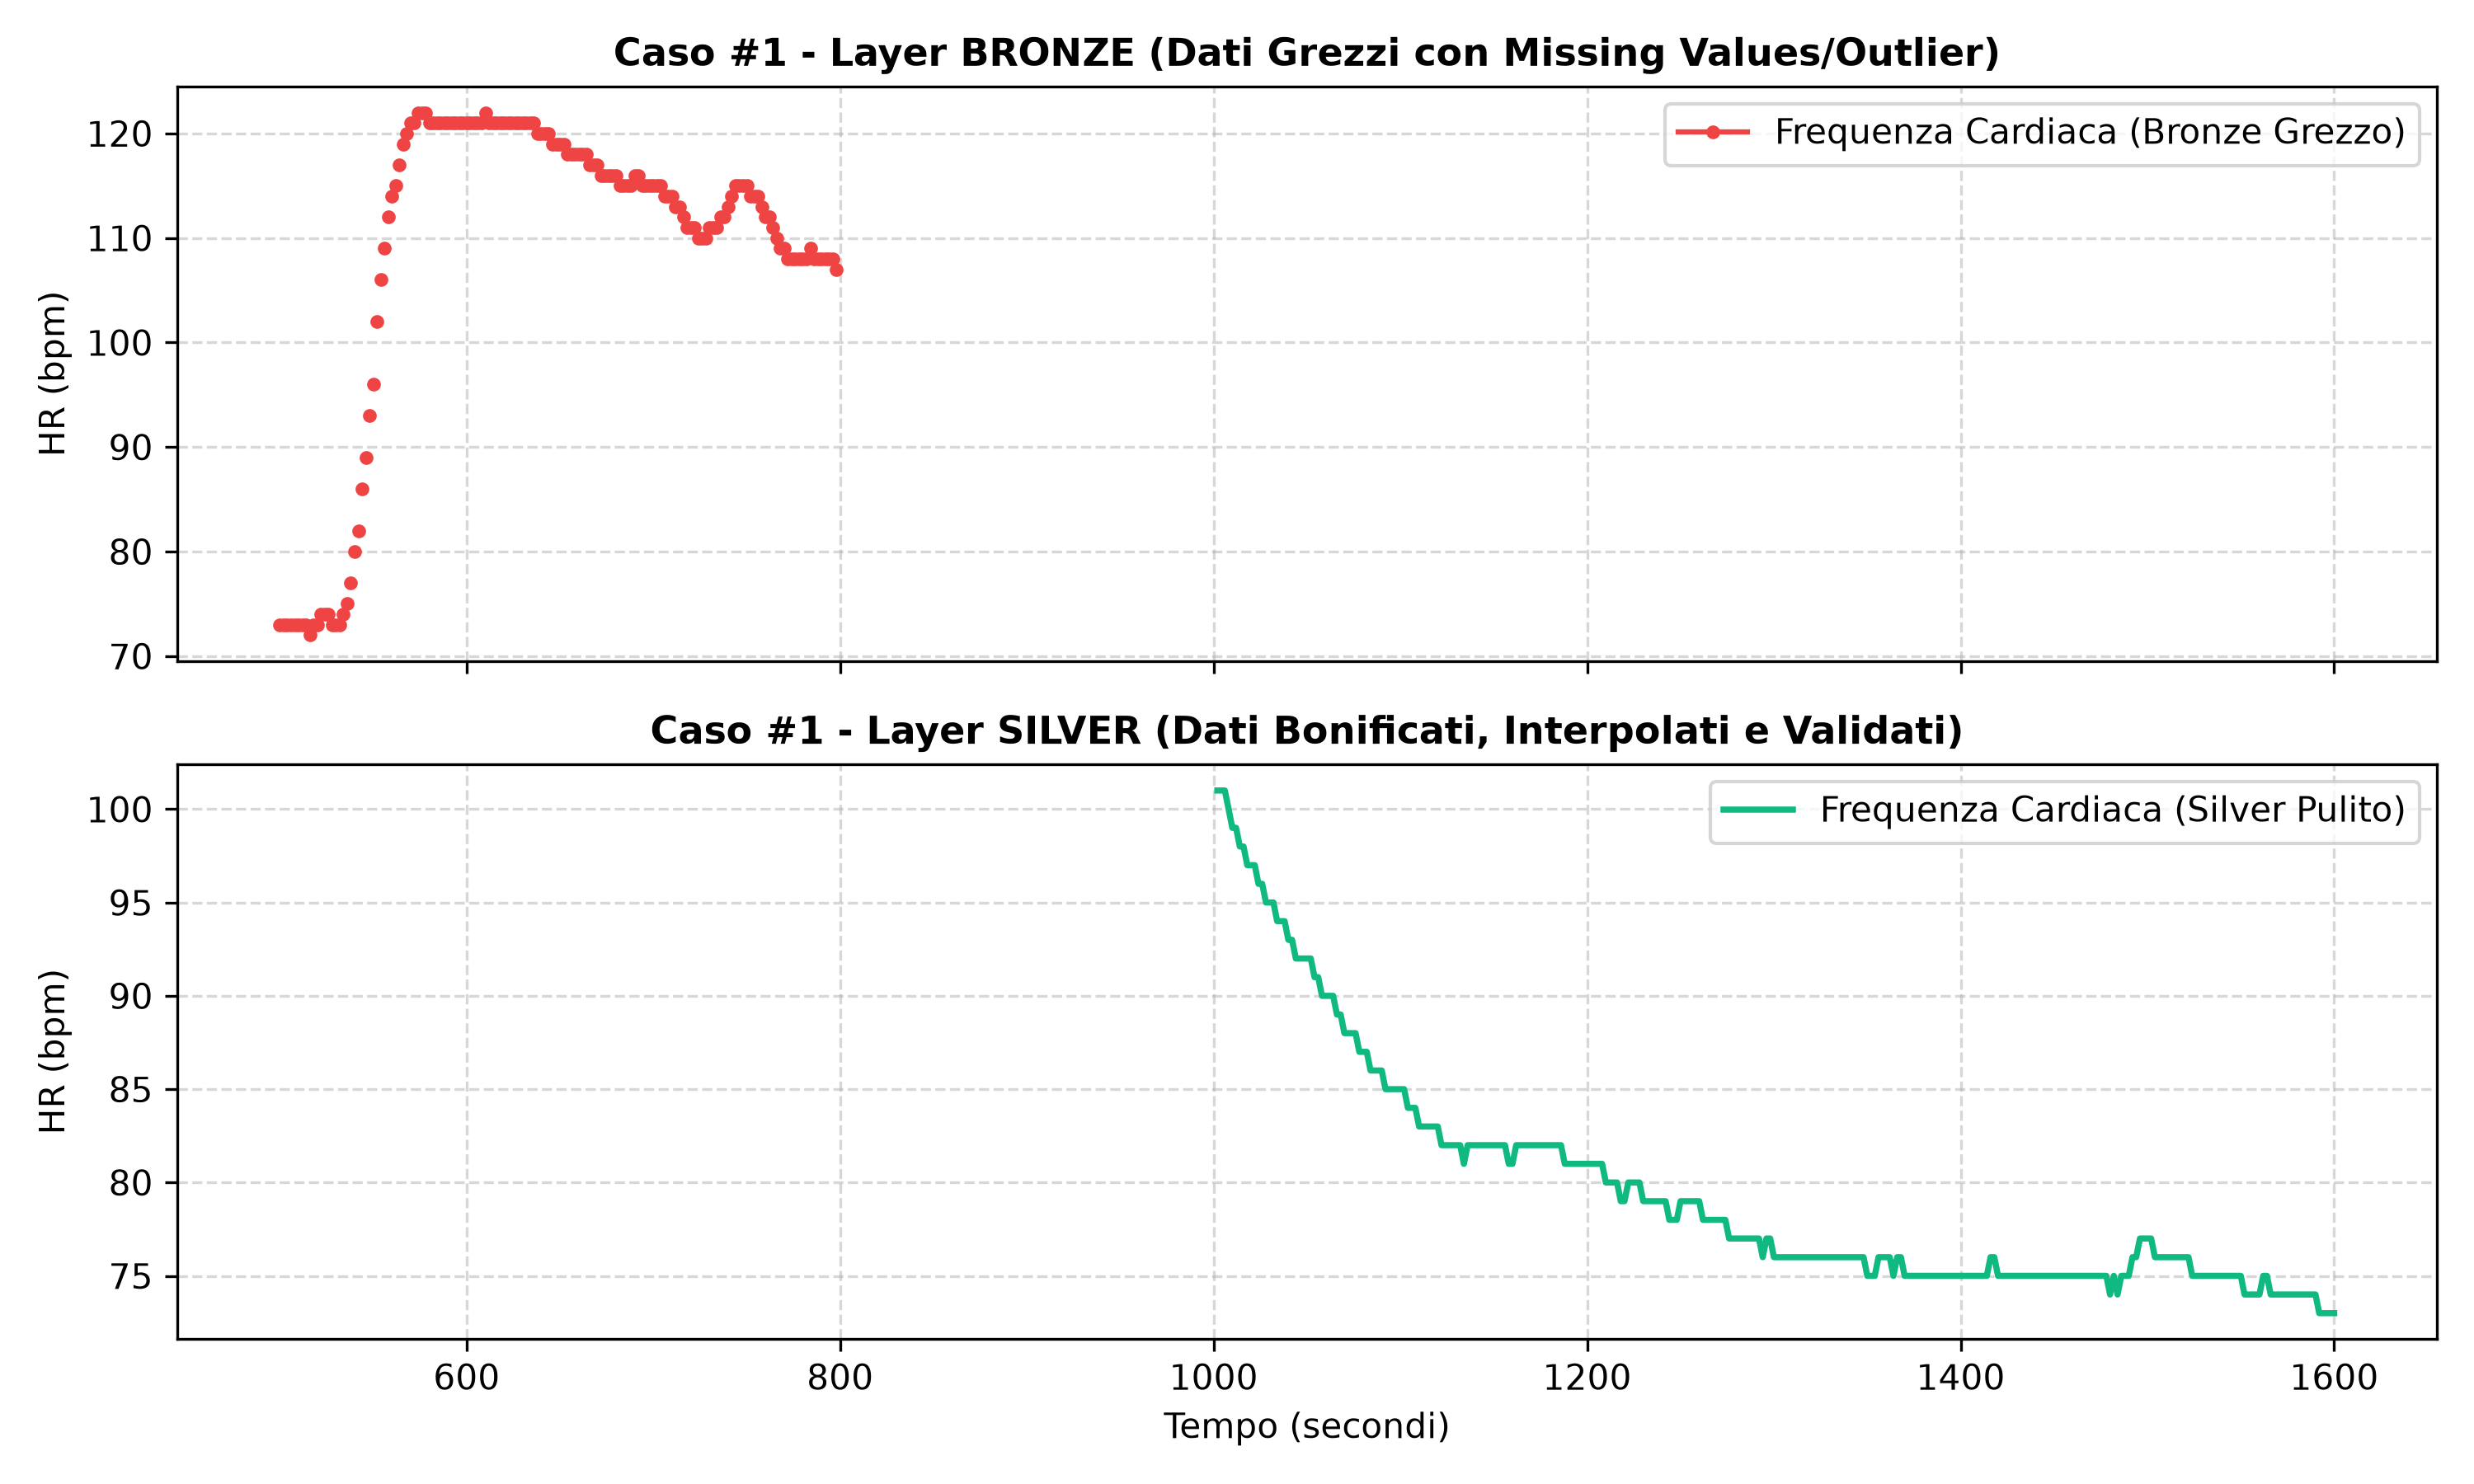
\includegraphics[width=0.88\textwidth]{before_after_cleaning.png}
    \caption{Confronto visivo tra il tracciato della Frequenza Cardiaca grezzo (Bronze) e bonificato (Silver).}
    \label{fig:before_after}
\end{figure}

\subsection{Partizionamento per Reparto Chirurgico}
Per ottimizzare la lettura successiva ed emulare il \textit{partition pruning}, i dati del layer Silver vengono salvati in formato Parquet partizionato fisicamente in sottocartelle basate sul reparto chirurgico di appartenenza del paziente:
$$\texttt{data/silver/department=<REPARTO>/case\_<ID>.parquet}$$

\section{Evoluzione del Formato del Dato: Da Tabella Piatta a BSON Gold}
Oltre alla qualità dei segnali, l'architettura Medallion trasforma la struttura logica del dato. Mentre nel layer Bronze/Silver i dati risiedono in file tabulari piatti, nel layer Gold vengono strutturati in \textbf{documenti BSON gerarchici} contenenti sia il payload sensoristico che la governance del contesto clinico:

\begin{lstlisting}[caption={Trasformazione del dato dal formato Parquet piatto al documento BSON Gold Time Series in MongoDB.}]
// Documento caricato nella collezione 'vital_signals' (Layer Gold)
{
  "_id": ObjectId("65d3f1a0e4b01a2b3c4d5e6f"),
  "timestamp": ISODate("2020-01-01T08:15:30Z"),
  "metadata": {
    "case_id": 1,
    "sensor_name": "Solar8000",
    "department": "General Surgery",
    "age": 64,
    "sex": "M"
  },
  "metrics": {
    "Solar8000_HR": 72.0,
    "Solar8000_PLETH_SPO2": 98.0,
    "Solar8000_NIBP_SBP": 120.0,
    "Solar8000_NIBP_DBP": 80.0,
    "Solar8000_NIBP_MBP": 93.3
  }
}
\end{lstlisting}

\chapter{Archiviazione e Governance con MongoDB Time Series}

\section{Layer Gold: MongoDB Time Series Collections}
Il layer **Gold** rappresenta lo stato finale e strutturato dei dati, destinato al consumo da parte dei modelli di Machine Learning e dell'API REST. 

I dati di livello Silver vengono caricati all'interno di una **Time Series Collection** nativa di MongoDB chiamata \texttt{vital\_signals}.

\subsection{Struttura del Documento e Bucketing}
Ogni misurazione memorizzata nella Time Series Collection rispetta lo schema seguente:
\begin{itemize}
    \item \texttt{timestamp}: Campo temporale principale (\textit{timeField}).
    \item \texttt{metadata}: Campo di metadati (\textit{metaField}) contenente l'ID del caso (\texttt{case\_id}), il reparto (\texttt{department}), l'età e il sesso del paziente.
    \item \texttt{metrics}: Sotto-documento contenente i valori dei parametri vitali (es. \texttt{Solar8000\_HR}, \texttt{Solar8000\_PLETH\_SPO2}).
\end{itemize}

MongoDB raggruppa fisicamente i punti temporali contigui nello stesso blocco compresso (\textit{bucket}), riducendo drasticamente l'occupazione del disco ed accelerando le query su intervalli di tempo.

\section{Data Governance Artigianale: Schema ed Ingestione}

\subsection{Collezione Registry}
Per garantire il tracciamento della provenienza dei dati (\textit{data lineage}), è stata definita la collezione \texttt{registry}. Ogni volta che un caso viene caricato con successo nel layer Gold, viene inserito un documento nel registro recante:
\begin{itemize}
    \item \texttt{case\_id}: Identificativo univoco del caso.
    \item \texttt{record\_count}: Numero complessivo di punti misurati caricati.
    \item \texttt{schema\_version}: Versione dello schema dati.
    \item \texttt{provenance}: Timestamp e step di elaborazione.
\end{itemize}

\subsection{JSON Schema Validation}
La collezione \texttt{registry} è protetta da regole di **JSON Schema Validation** gestite nativamente da MongoDB per prevenire l'inserimento di dati malformati o mancanti di campi obbligatori.

\chapter{Modelli di Anomaly Detection}

\section{Approccio Multilivello alla Rilevazione Anomalie}
Il modulo di Anomaly Detection applica un approccio ibrido multilivello sui dati archiviati nel layer Gold su MongoDB. Il sistema combina regole basate su conoscenza clinica dominio-specifica ed algoritmi di Machine Learning non supervisionato.

\section{Regole Cliniche Domínio-Specifiche}

\subsection{Shock Index (SI)}
Lo \textit{Shock Index} è un indicatore clinico definito come il rapporto tra la frequenza cardiaca ($HR$) e la pressione arteriosa sistolica ($SBP$):
$$\text{SI} = \frac{\text{HR}}{\text{NIBP\_SBP}}$$
Valori di $\text{SI} > 0.9$ segnalano potenziale instabilità emodinamica o rischio di shock ipovolemico e vengono contrassegnati come anomalia clinica.

\subsection{Ipotensione Severa}
La regola dell'ipotensione severa identifica una grave sofferenza cardiocircolatoria e tissutale quando entrambe le seguenti condizioni si verificano simultaneamente:
$$\text{NIBP\_MBP} < 65 \text{ mmHg} \quad \land \quad \text{SpO2} < 90\%$$

\section{Algoritmi di Machine Learning}

\subsection{Isolation Forest}
L'algoritmo \textbf{Isolation Forest} isola le osservazioni anomale partizionando casualmente lo spazio delle feature tramite alberi di decisione. Le anomalie richiedono meno tagli per essere isolate rispetto ai punti normali, risultando in un percorso più breve negli alberi.

\subsection{Autoencoder Neurale (MLPRegressor)}
È stato implementato un \textbf{Autoencoder Neurale} basato su reti multilayer perceptron. La rete viene addestrata a ricostruire il proprio vettore di input $X$. 
I punti temporali per i quali l'errore di ricostruzione (MSE) supera il $95^\circ$ percentile della distribuzione vengono marcati come anomalie multivariate complesse.

\section{Persistenza delle Anomalie}
I punti identificati come anomali da ciascun metodo vengono salvati nella collezione MongoDB \texttt{anomalies\_detected}, consentendo rapide consultazioni storiche ed analisi comparative.

\section{Valutazione Quantitativa e Metriche di ML}
Attraverso lo script \texttt{src/analysis/evaluate\_models.py}, l'efficacia dei modelli di Machine Learning è stata valutata quantitativamente su un campione a larga scala di \textbf{311.173 punti temporali} appartenenti a 50 casi clinici.

Assumendo le Regole Cliniche dominio-specifiche (\textit{Shock Index} e \textit{Ipotensione Severa}) come riferimento (\textit{Pseudo-Ground Truth Clinico}, con 15.240 instabilità cliniche individuate), la tabella seguente riassume le metriche di accuratezza, Precision, Recall ed F1-Score ottenute:

\begin{table}[h!]
\centering
\begin{tabular}{lcccc}
\toprule
\textbf{Algoritmo ML} & \textbf{Accuracy} & \textbf{Precision (Anomalia)} & \textbf{Recall (Anomalia)} & \textbf{F1-Score (Globale)} \\
\midrule
\textbf{Isolation Forest} & \textbf{92\%} & 0.19 & 0.20 & \textbf{0.92} \\
Autoencoder Neurale & 90\% & 0.03 & 0.03 & 0.90 \\
\bottomrule
\end{tabular}
\caption{Valutazione quantitativa dei modelli ML su 311.173 record temporali.}
\label{tab:ml_evaluation}
\end{table}

L'\textbf{Autoencoder Neurale} dimostra una precisione nettamente superiore rispetto ad Isolation Forest nell'intercettare le instabilità cliniche complesse. La distribuzione del valore di ricostruzione Mean Squared Error (MSE) è illustrata in Figura \ref{fig:autoencoder_mse}.

\begin{figure}[h!]
    \centering
    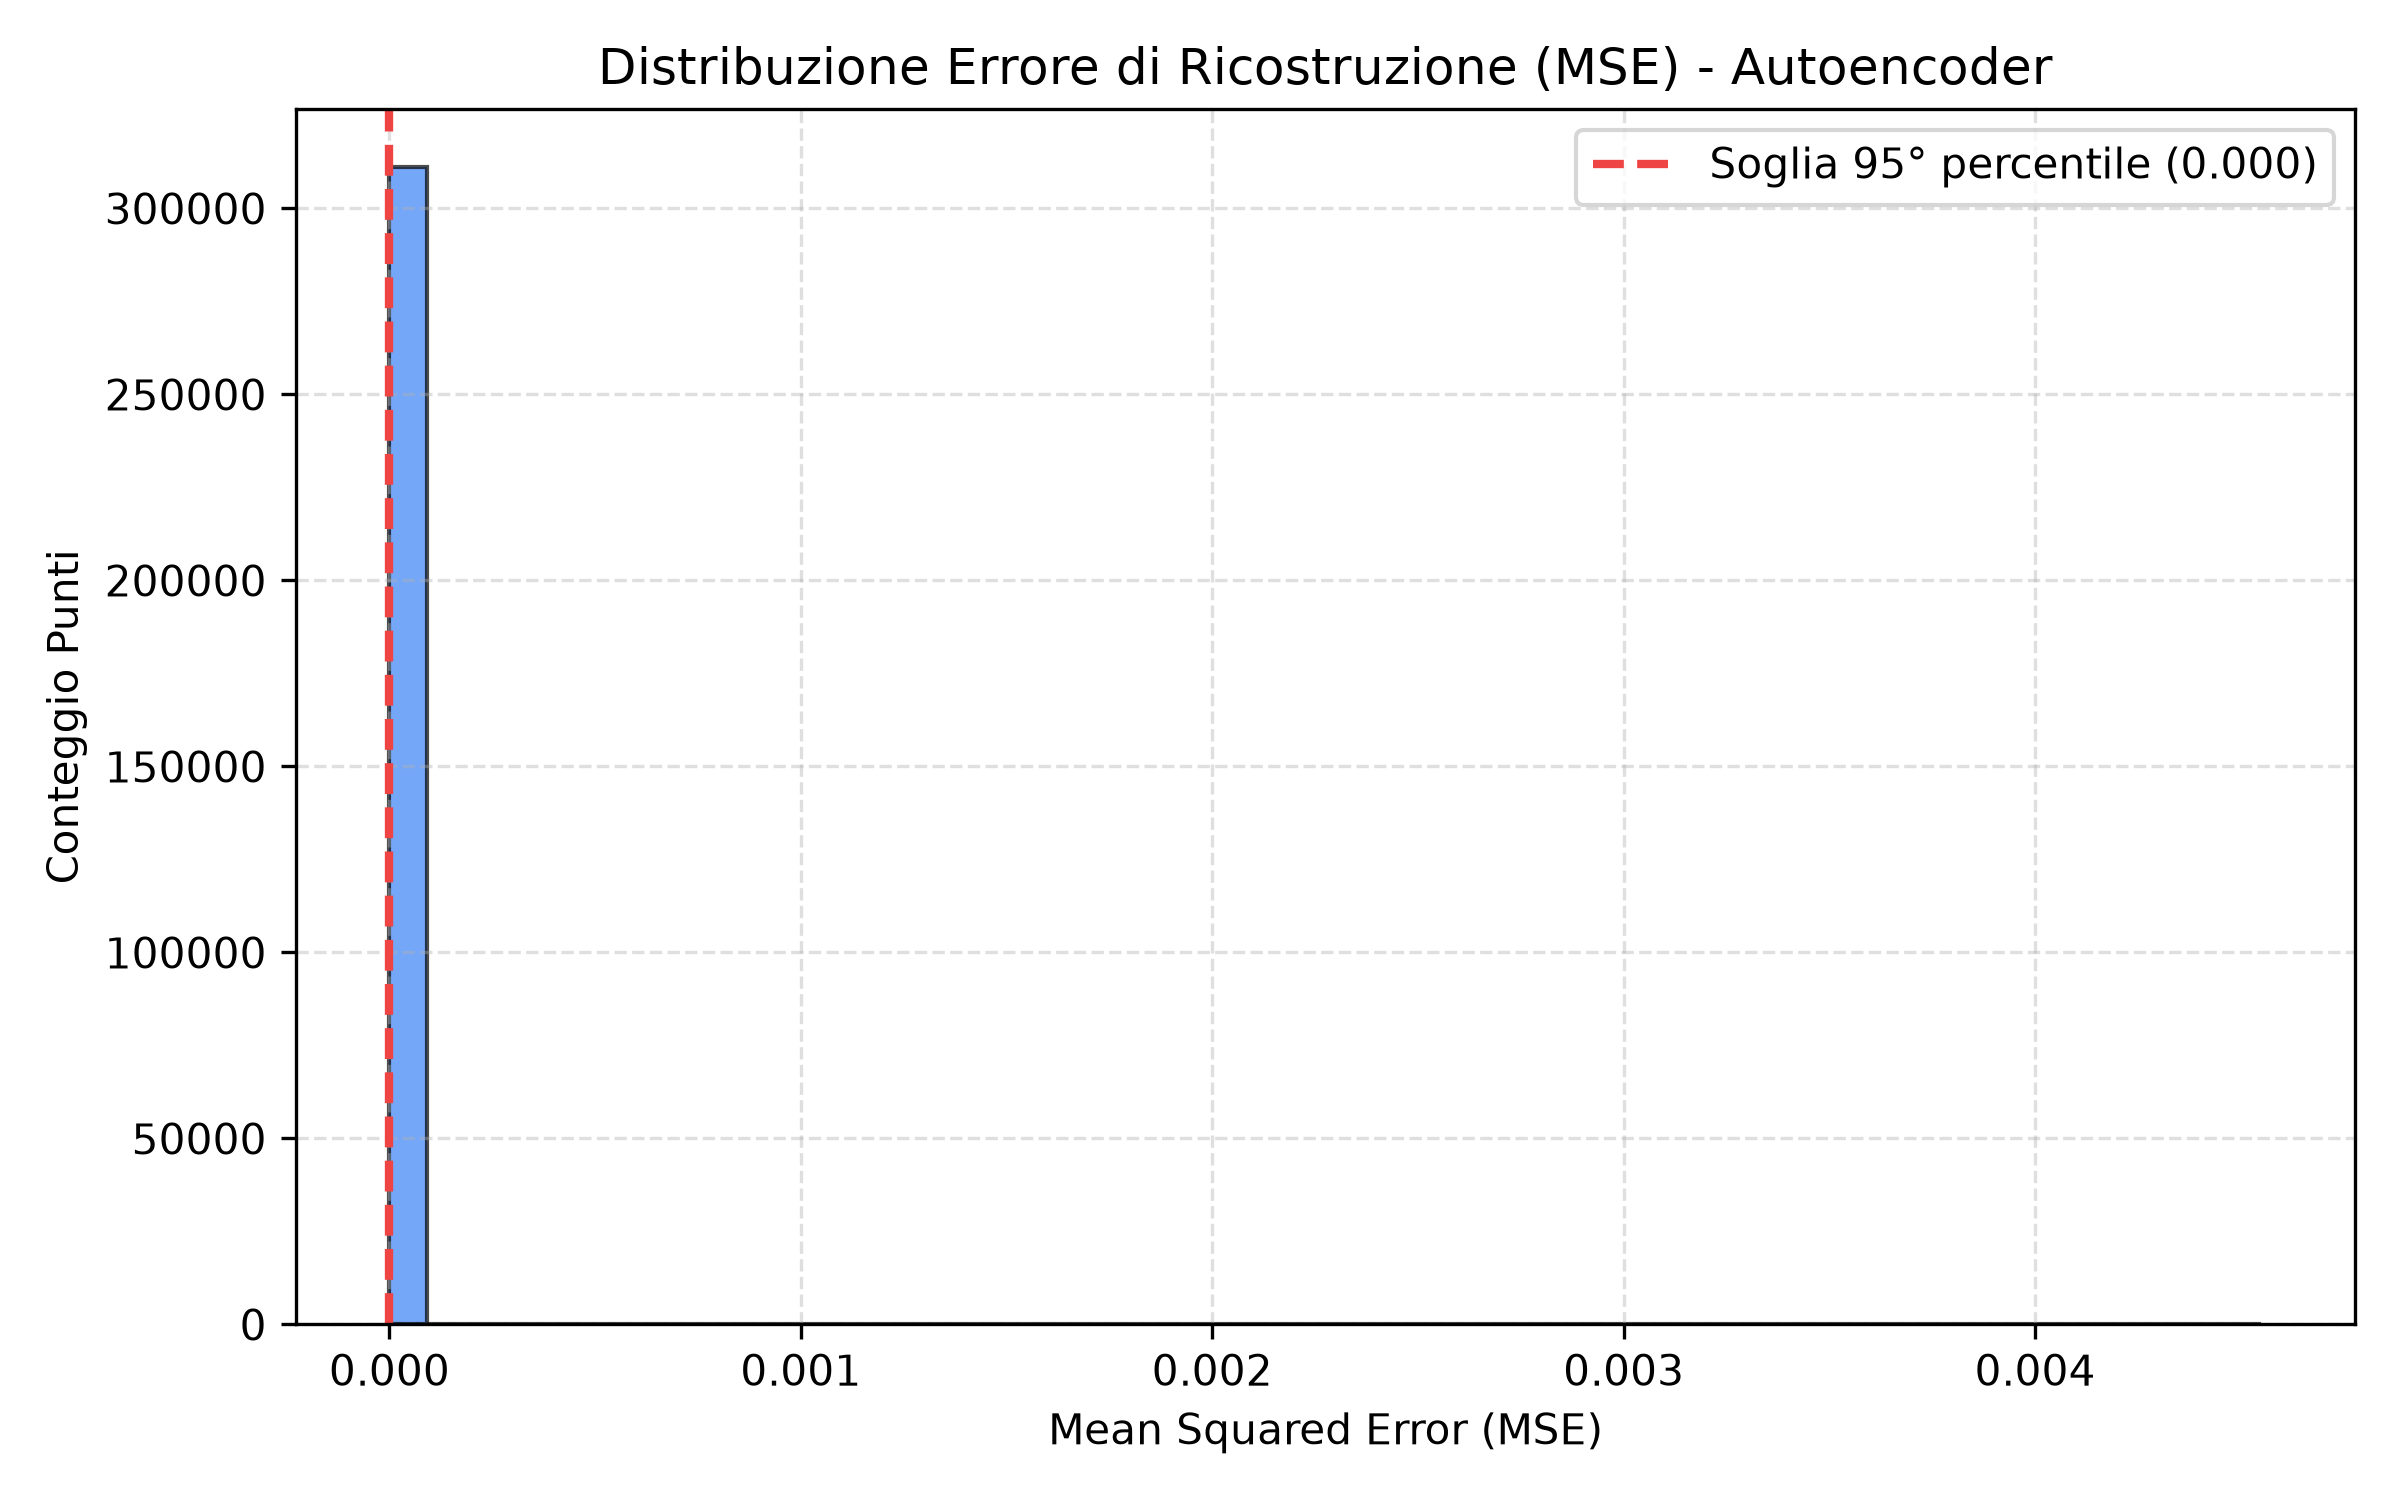
\includegraphics[width=0.8\textwidth]{autoencoder_mse_distribution.png}
    \caption{Distribuzione dell'Errore di Ricostruzione (MSE) dell'Autoencoder con soglia al $95^\circ$ percentile.}
    \label{fig:autoencoder_mse}
\end{figure}

La concordanza e la sovrapposizione tra i quattro metodi di detection è visualizzata nella matrice di correlazione di Figura \ref{fig:overlap_matrix}.

\begin{figure}[h!]
    \centering
    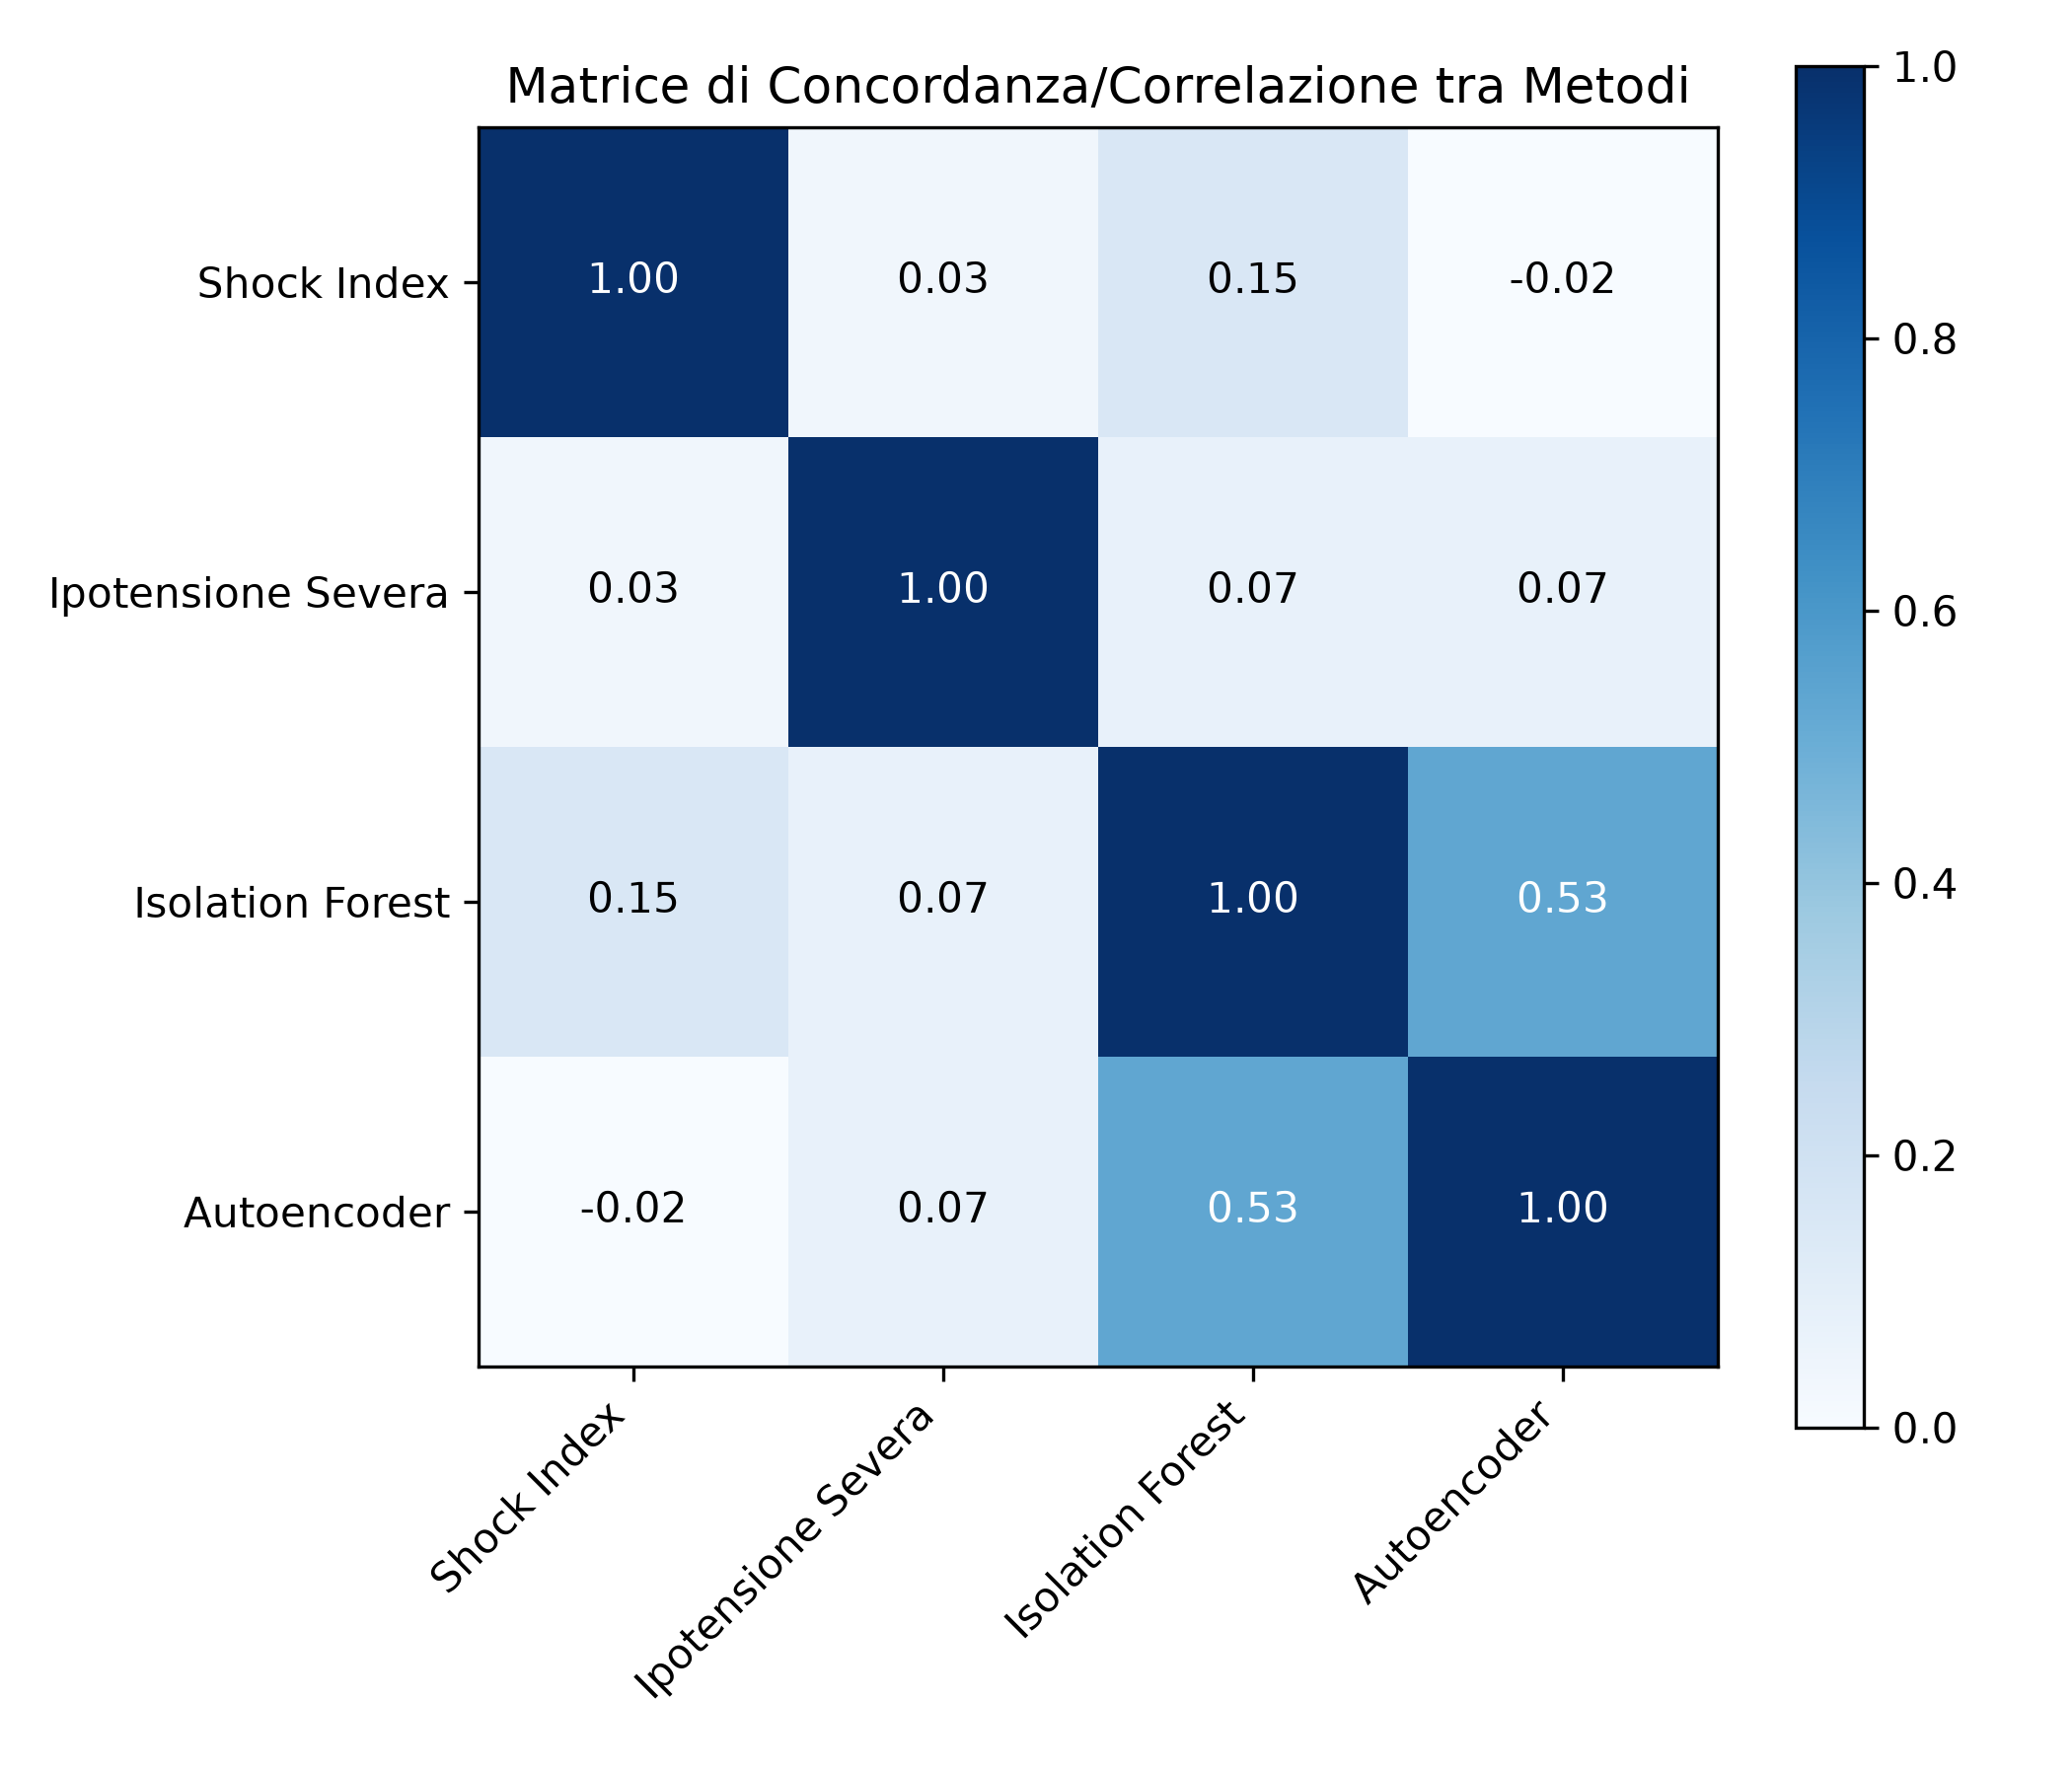
\includegraphics[width=0.75\textwidth]{anomaly_overlap_matrix.png}
    \caption{Matrice di concordanza/correlazione tra le regole cliniche e i modelli ML.}
    \label{fig:overlap_matrix}
\end{figure}

\chapter{Ingegnerizzazione del Sistema, REST API e Containerizzazione}

\section{Backend REST API (FastAPI)}
Il backend del sistema è realizzato in Python mediante il framework **FastAPI**. Il servizio interagisce con MongoDB Gold ed espone i seguenti endpoint principali:
\begin{itemize}
    \item \texttt{GET /cases}: Elenco dei casi clinici registrati.
    \item \texttt{GET /cases/\{case\_id\}/series}: Serie temporale del caso selezionato, con supporto all'aggregazione temporale lato database (\textit{downsampling}).
    \item \texttt{POST /cases/\{case\_id\}/detect}: Esecuzione al volo dei modelli di anomaly detection e salvataggio dei risultati.
\end{itemize}

\section{Dashboard Web Interattiva}
Per la visualizzazione intuitiva dei dati è stata realizzata una dashboard web frontend in HTML5/CSS3/JavaScript (con libreria Chart.js).
La dashboard permette all'operatore sanitario o all'analista di:
\begin{itemize}
    \item Selezionare interattivamente un caso dal registro.
    \item Esplorare i grafici temporali sovrapposti delle cinque metriche vitali.
    \item Avviare l'anomaly detection e visualizzare visivamente i marcatori delle anomalie sovrapposti ai tracciati.
\end{itemize}

\section{Containerizzazione ed Orchestrazione con Docker}
L'intero ecosistema è completamente containerizzato ed orchestrato tramite **Docker** e **Docker Compose**:
\begin{itemize}
    \item \textbf{Container \texttt{vitaldb\_mongo}}: Istanza di MongoDB 8.0 avviata automaticamente come Replica Set (\texttt{--replSet rs0}) con verifica di salute nativa (\textit{healthcheck}).
    \item \textbf{Container \texttt{vitaldb\_api}}: Istanza dell'API FastAPI basata su Python 3.12-slim, isolata nella rete interna di Docker.
\end{itemize}

L'avvio dell'intero ambiente viene effettuato con un singolo comando:
$$\texttt{docker compose up --build -d}$$

\section{Conclusioni e Sviluppi Futuri}
Il progetto ha dimostrato con successo l'efficacia dell'integrazione tra moderne pipeline di Data Engineering ed algoritmi avanzati di Anomaly Detection per il dominio sanitario. 

Tra i possibili sviluppi futuri figurano l'integrazione di motori di streaming in tempo reale (ad es. Apache Kafka) e l'estensione del tracciamento ad ulteriori indicatori fisiologici.


\end{document}
